\section{Static Interface Design}
\label{sect:static_interface_design}

Mock-ups of key views were created using Balsamiq~\cite{BALSAMIQ_MOCKUPS_3:1}~to illustrate the desired user interface associated with these windows prior to finalized implementation.

\subsection{Sign-in Window}
\label{sect:signin_window}

Figure \ref{fig:signin} shows a mock-up of the login window for PyBank. The icon shown is a current placeholder until a finalized logo for the application can be developed. Password will display a masked version of the entered password for user privacy; however, when holding the eye shaped icon down, the password will show for the user. There is a link to sign-up available, button to sign up, and a button to cancel login and exit the application.

\FloatBarrier
\begin{figure}[!ht]
    \centering
    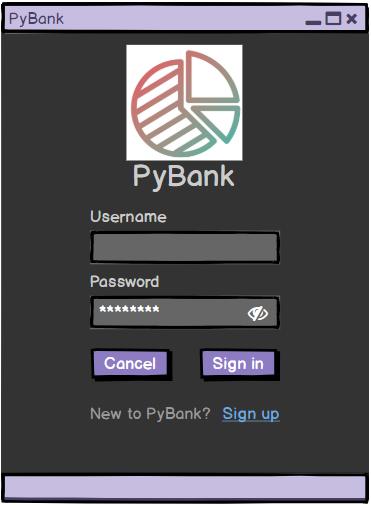
\includegraphics[width=8cm]{figures/signin.png}
    \caption{The Sign-in window for PyBank.}
    \label{fig:signin}
\end{figure}

\newpage

\subsection{Sign-up Window Part II}
\label{sect:signup_window}

Figure \ref{fig:signup} is a mock-up of the second part of the sign-up window. Along the top is a progress bar, showing the user where in the sign-up process they are. Below the progress bar is a title, describing the purpose of the current step in the process. On this window, the user can utilize the checkbox that will grey out all options below besides next and back, keeping the user from entering information and allowing them to skip the window. Otherwise, the user may choose to link a bank account from a partnered bank, or enter account information manually for the user to track finances without linking all information.

\FloatBarrier
\begin{figure}[!ht]
    \centering
    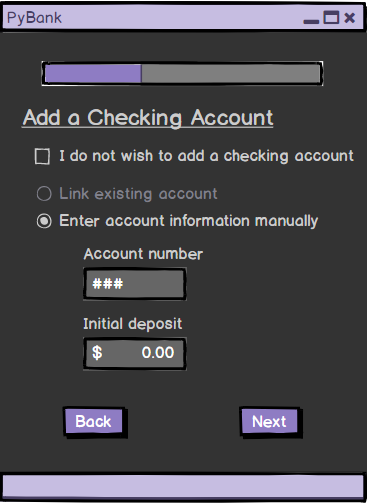
\includegraphics[width=8cm]{figures/signup.png}
    \caption{The Sign-up window part II for PyBank.}
    \label{fig:signup}
\end{figure}

\newpage

\subsection{Account Overview Window}
\label{sect:acct_overview}

Figure \ref{fig:overview} is the account overview. This window provides a brief summary of account information for the user to access at a glance. This includes account balances, account number--which is entered by the user and serves as a form of account identification in the event the user has multiple of the same type of account—and an overview of the most recent transactions. Because this was the most common functionality utilized by stakeholders, it is the first window the user is taken to after signing in.

\FloatBarrier
\begin{figure}[!ht]
    \centering
    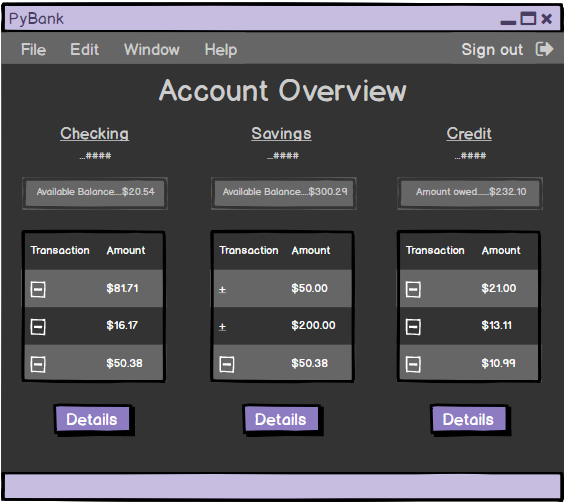
\includegraphics[width=11cm]{figures/accountoverview.png}
    \caption{The account overview window shows basic information relating to all accounts owned by the user.}
    \label{fig:overview}
\end{figure}

\newpage

\subsection{Checking Account Window}
\label{sect:checking_acct}

Figure \ref{fig:details} is the account details window. This window serves to show transaction details, upcoming bills, and a bill calendar. There is a search functionality as well that allows the users to find a specific transaction or bill. Along the top, this window provides options to access graph displays, send money, or transfer money.

\FloatBarrier
\begin{figure}[!ht]
    \centering
    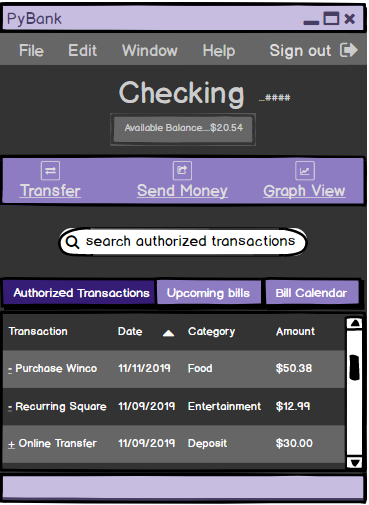
\includegraphics[width=8cm]{figures/accountdetails.png}
    \caption{A detailed view of a specific account's checking account details.}
    \label{fig:details}
\end{figure}

\newpage

\subsection{Online Transfer Funds Window}
\label{sect:online_transfer_funds}

The window for performing online transfers is shown in Figure \ref{fig:transfer}. In this view, the user selects an account from the drop down menu to dictate where money is to be transferred from and where it is to be transferred to. The user then enters a value to transfer between accounts and the date on which the transfer is to take place.

\FloatBarrier
\begin{figure}[!ht]
    \centering
    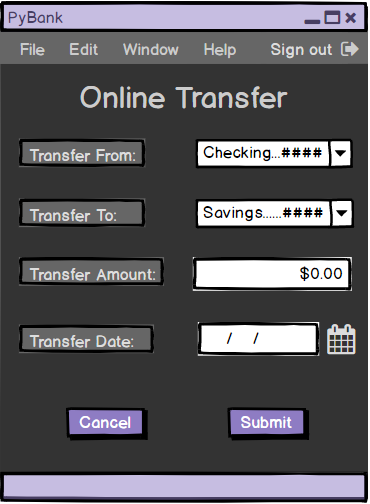
\includegraphics[width=8cm]{figures/transfer.png}
    \caption{A detailed view of a specific account performing an online transfer.}
    \label{fig:transfer}
\end{figure}

\newpage

\subsection{Visualization Window}
\label{sect:visualization_window}

Graphical representations of finances and budgeting are shown in Figure \ref{fig:graphs}. This view allows an alternate was to be able to see summaries of important information to the user. Along the top of the screen is the current graph being displayed. Below that is a set of radio buttons where the user is able to pick from a list of different graphs.

\FloatBarrier
\begin{figure}[!ht]
    \centering
    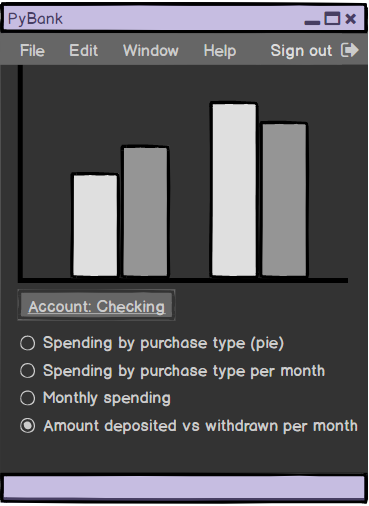
\includegraphics[width=8cm]{figures/accountgraphs.png}
    \caption{A detailed view of a specific account's visualizations.}
    \label{fig:graphs}
\end{figure}

\FloatBarrier
%EOF